\chapter{Detección de intrusiones} \label{Capitulo4}

En la era actual, Internet se ha convertido en una herramienta esencial en nuestra vida cotidiana, facilitando actividades en áreas como los negocios, el entretenimiento y la educación \citep{tsai2009intrusion}. Sin embargo, esta tendencia también ha acarreado un mayor riesgo de ataques en la red, lo que subraya la necesidad de sistemas de seguridad mas potentes. Para garantizar la seguridad de las redes, es esencial contar con sistemas de detección de intrusiones capaces de identificar estos ataques (IDS, por sus siglas en inglés) \citep{liu2019machine}.


La detección de anomalías se centra en identificar desviaciones de los patrones normales de uso, asumiendo que tales desviaciones pueden representar intentos de intrusión. Estos sistemas han evolucionado significativamente, incorporando técnicas avanzadas de aprendizaje automático para identificar diferencias entre datos anómalos y benignos con alta precisión. Además, estas técnicas han demostrado ser efectivas para manejar grandes volúmenes de datos y mejorar la capacidad de detección de nuevos tipos de ataques \citep{liu2019machine}.

En este capítulo vamos a enfrentar este problema, escogiendo una de las bases de datos disponibles en \citep{podder2021artificial} para poder identificar intrusiones. Como el objetivo principal de este trabajo es el estudio y puesta en práctica de diferentes algoritmos de aprendizaje automático, se ha decidido tomar como base de datos \textit{KDD CUP 1999} \citep{kddcup99}, uno de los conjuntos de datos más utilizados para evaluar sistemas de detección de intrusiones. Otro de los motivos de esta elección ha sido la gran variedad de métodos que están documentados en el review para poder resolverlo, en particular de cuatro formas diferentes. Usando una \acrfull{cnn}, una \acrfull{dnn}, una \acrfull{rnn} y un \textit{autoencoder}. 




\section{KDD Cup 1999 Data}

La base de datos\textit{ KDD CUP 1999} se desarrolló a partir de un conjunto de datos recopilado durante el Programa de Evaluación de Detección de Intrusiones DARPA de 1998, gestionado por los Laboratorios Lincoln del MIT (\textit{Massachusetts Institute of Technology}). Este programa tenía como objetivo evaluar métodos de detección de intrusiones mediante la simulación de ataques en una red de área local (LAN) que imitaba el entorno de un área de la Fuerza Aérea de EE.UU \citep{kddcup99}.

\newpage

Para crear el conjunto de datos, los Laboratorios Lincoln capturaron datos de TCP durante nueve semanas en esta red simulada. El conjunto de datos de entrenamiento incluye aproximadamente siete semanas de tráfico de red comprimido en cuatro \textit{Gbytes} de datos binarios, procesados en unos cinco millones de registros de conexión. Los datos de prueba abarcan dos semanas adicionales y contienen alrededor de dos millones de registros de conexión \citep{kddcup99}.

Una conexión en el conjunto de datos se define como una secuencia de paquetes TCP entre una dirección IP de origen y una dirección IP de destino, con un inicio y fin definidos. Cada conexión está etiquetada como normal o como un ataque, con uno de los varios tipos específicos de ataque. Este enfoque permite analizar el comportamiento de las conexiones en un entorno controlado y detectar patrones asociados con actividades maliciosas \citep{kddcup99}.

En \citep{kddcup99} nos encontramos con los siguientes archivos:

\begin{itemize}
    \item \textit{taskdescription}: Esta es la descripción original de la tarea proporcionada a los participantes de la competencia.
    \item \textit{kddcup.names}: Una lista de características.
    \item \textit{kddcup.data.gz}: El conjunto de datos completo (18M; 743M sin comprimir).
    \item \textit{kddcup.data\_10\_percent.gz}: Un subconjunto del 10\% (2.1M; 75M sin comprimir).
    \item \textit{kddcup.newtestdata\_10\_percent\_unlabeled.gz}: Un subconjunto del 10\% de datos de prueba sin etiquetas (1.4M; 45M sin comprimir).
    \item \textit{kddcup.testdata.unlabeled.gz}: Datos de prueba sin etiquetas (11.2M; 430M sin comprimir).
    \item \textit{kddcup.testdata.unlabeled\_10\_percent.gz}: Un subconjunto del 10\% de datos de prueba sin etiquetas (1.4M; 45M sin comprimir).
    \item \textit{training\_attack\_types}: Una lista de tipos de intrusión.
    \item \textit{typo-correction.txt}: Una breve nota sobre un error tipográfico en el conjunto de datos que ha sido corregido (26/6/07).
\end{itemize}

En este caso, utilizaremos únicamente el conjunto de datos \textit{kddcup.data.gz} para hacer nuestros experimentos ya que necesitamos saber si una instancia es buena o mala para entrenarla en nuestras redes neuronales. 

Cada registro del conjunto de datos contiene 41 características diferentes, las cuales se puede ver su descripción en la tabla \ref{tab: caracKDD}. Además, contiene una característica final con el nombre con el que se clasifica la instancia. Podemos visualizar un ejemplo de como nos aparecen las instancias en el archivo \textit{kddcup.data.gz} en la figura \ref{img: kddpreview}. Estas características se dividen en tres grupos principales: características de tráfico, características de conexión TCP y características de contenido.
\begin{figure}[h]
    \begin{center}
    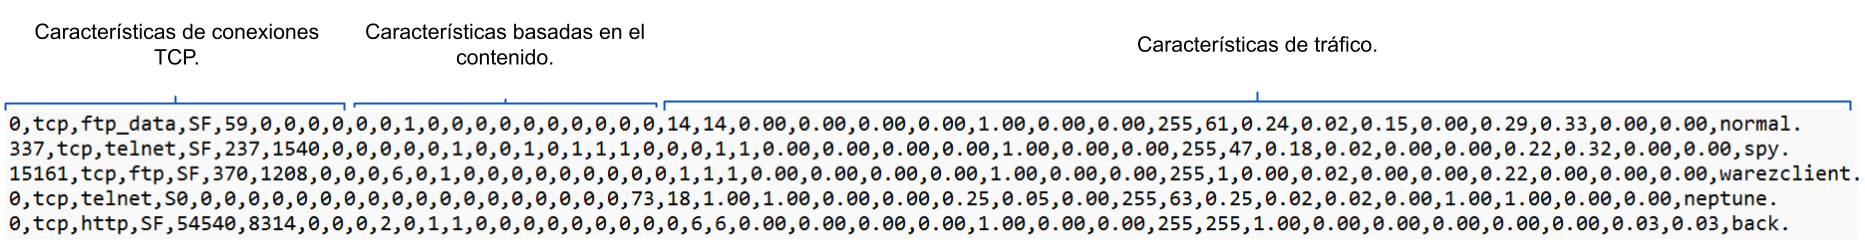
\includegraphics[width=\textwidth]{img/kddpreview.png}
    \end{center}
    \caption{Visualización del archivo \textbf{kddcup.data.gz}.}
    \label{img: kddpreview}
\end{figure}

\newpage


\begin{table}[h!]
    \centering
    \begin{tabular}{|c|l|l|}
        \hline
        \textbf{No.} & \textbf{Descripción} & \textbf{Tipo} \\
        \hline
        \multicolumn{3}{|c|}{\textbf{Características de Conexiones TCP}} \\
        \hline
        1 & duración de la conexión (s) & int64 \\
        2 & tipo protocolo & str \\
        3 & tipo servicio red destino & str \\
        4 & estado de la conexión & str \\
        5 & bytes origen-destino & int64 \\
        6 & bytes destino-origen & int64 \\
        7 & 1 si puerto/host similar, 0 otro caso & int64 \\
        8 & fragmentos incorrectos & int64 \\
        9 & paquetes urgentes & int64 \\
        \hline
        \multicolumn{3}{|c|}{\textbf{Características de Contenido}} \\
        \hline
        10 & indicaciones calientes & int64 \\
        11 & intentos de inicio de sesión fallidos & int64 \\
        12 & 1 si inicio de sesión aceptado & int64 \\
        13 & operaciones comprometidas & int64 \\
        14 & 1 si acceso root en shell & int64 \\
        15 & invocación de su root & int64 \\
        16 & accesos concedidos como root & int64 \\
        17 & creaciones de archivos & int64 \\
        18 & sesiones de shell & int64 \\
        19 & operaciones de acceso a archivos & int64 \\
        20 & instrucciones salientes en ftp & int64 \\
        21 & 1 si inicio de sesión es de host & int64 \\
        22 & 1 si inicio de sesión como invitado & int64 \\
        \hline
        \multicolumn{3}{|c|}{\textbf{Características de Tráfico}} \\
        \hline
        23 & enlaces en 2s al mismo host & int64 \\
        24 & enlaces en 2s al mismo servicio & int64 \\
        25 & \% fallos SYN & float64 \\
        26 & \%  conexiones hacia mismo servicio con errores SYN & float64 \\
        27 & \% fallos REJ & float64 \\
        28 & \%  conexiones hacia el mismo servicio que tuvieron errores REJ & float64 \\
        29 & \% conexiones a un solo servicio & float64 \\
        30 & \% conexiones a varios servicios & float64 \\
        31 & \% conexiones a varios hosts & float64 \\
        32 & conexiones al mismo host de destino & int64 \\
        33 & conexiones al mismo servicio & int64 \\
        34 & \% conexiones al mismo host & float64 \\
        35 & \% conexiones varios servicios & float64 \\
        36 & \% conexiones mismo puerto de origen & float64 \\
        37 & \% conexiones varios hosts al mismo servicio & float64 \\
        38 & \% conexiones fallos S0 al host actual & float64 \\
        39 & \% conexiones fallos S0 al host y servicio & float64 \\
        40 & \% fallos RST al host actual & float64 \\
        41 & \% fallos RST al host y servicio & float64 \\
        42 & tipo de ataque & str \\
        \hline
    \end{tabular}
    \caption{Características del Conjunto de Datos KDD}
    \label{tab: caracKDD}
\end{table}

\begin{itemize}
    \item \textbf{Características de conexiones TCP}: Examina las características que describen los atributos básicos de cada conexión TCP.
    \item \textbf{Características basadas en el contenido}: Estas características examinan el contenido de los paquetes para identificar patrones sospechosos.
    \item \textbf{Características de tráfico}: Estas características analizan patrones de tráfico en la red para detectar anomalías.
\end{itemize}


El conjunto de datos de entrenamiento del \textit{KDD Cup 1999} comprenden diferentes formas de amenazas y datos normales. Cada uno de los datos anómalos pertenecen a una de las siguientes 22 formas diferentes de ciberataques (ver tabla \ref{tab: catKDD}). Estos ataques pueden clasificarse en 4 grupos, que según \citep{arief2022comparison}, podemos describirlos como:
\begin{itemize}
    \item \textbf{Ataque de Denegación de Servicio (DoS)}: ocurre cuando un intruso impide que los usuarios autorizados accedan a un sistema sobrecargando los recursos del sistema (computación o memoria), haciéndolo incapaz de ejecutar solicitudes válidas, como en el caso de una inundación SYN.
    \item \textbf{Ataque de Usuario a Root (U2R)}: ocurre cuando el intruso obtiene permisos locales para acceder al sistema como un usuario legítimo y luego intenta explotar debilidades para obtener acceso root al sistema, ganando así capacidades de supervisión.
    \item \textbf{Ataque de Remoto a Local (R2L)}: ocurre cuando el intruso transmite un paquete a través de la red desde una estación de trabajo remota sin proporcionar el permiso adecuado, como al intentar varias contraseñas.
    \item \textbf{Ataque de Sondeo}: ocurre cuando un intruso intenta obtener conocimiento sobre la red para descubrir fallos de seguridad. A través de esta operación, el intruso explora la arquitectura de la red e identifica las categorías de servicios disponibles en el sistema utilizando técnicas como un escaneo de puertos.
\end{itemize}

En la tabla \ref{tab: catKDD} podemos ver los tipos de ataque que incluye cada grupo y el número total de muestras que tiene.

\begin{table}[h!]
    \centering
    \begin{tabular}{|l|l|c|}
        \hline
        \textbf{Categoría} & \textbf{Ataque} & \textbf{Total}\\
        \hline
        DOS & pod, land, neptune, smurf, teardrop, back & 3.883.370\\
        R2L & warezclient, imap, phf, spy, ftpwrite, guesspswd, warezm, multihop & 1.126\\
        U2R & rootkit, loadmodule, perl, buffer\_ overflow & 52\\
        Probing & satan, nmap, portsweep, ipsweep & 41.102\\
        Normal & & 972.781 \\
        \hline
    \end{tabular}
    \caption{Categorías de Ataques}
    \label{tab: catKDD}
\end{table}


El propósito de la competición \textit{KDD Cup 1999}, en la cual se utilizó este conjunto de datos, era desarrollar un modelo predictivo capaz de distinguir entre conexiones normales y ataques \citep{kddcup99}. Este conjunto de datos se ha convertido en una referencia clave en estudios sobre la detección de intrusiones en redes debido a su riqueza y diversidad de ejemplos de ataques.



\section{Preparación datos} \label{sec:datoskdd}

De estas 41 características de tráfico, 38 son numéricas y 3 son simbólicas. Para unificar los formatos de datos, transformamos las características simbólicas en datos numéricos utilizando vectores \emph{one-hot}. Las 3 características simbólicas son: el tipo de protocolo en la capa TCP/IP, el tipo de servicio del sistema objetivo, y el tipo de bandera que indica el estado de la conexión de la sesión. Tenemos tres tipos de protocolos, ICMP, TCP, y UDP. Estos protocolos se transforman en un vector de tres dimensiones, resultando en las representaciones (1,0,0), (0,1,0) y (0,0,1) respectivamente. De manera similar, los 70 tipos de servicio, que incluyen HTTP y FTP, se transforman en vectores de 70 dimensiones, y las 11 características de tipo de bandera se convierten en vectores de 11 dimensiones. A través de estas transformaciones, generamos un vector de 84 dimensiones, que al combinar con las 38 características originales numéricas, obtenemos un vector final de 122 dimensiones.

Además, cada valor lo estandarizamos utilizando la siguiente fórmula:
\begin{equation}
    X_{inorm} = \frac{x_i-x_{imin}}{x_{imax}-x_{imin}}
\end{equation}

donde $X_{inorm} \in \mathbb{R}$ hace referencia al nuevo valor normalizado, $x_i \in \mathbb{R}$ al valor que se encuentra en la base de datos y $x_{imax}$, $x_{imin} \in \mathbb{R}$ al valor máximo y mínimo de esa característica respectivamente. De esta forma, todas las características se van a encontrar entre $[0,1]$ \citep{kim2018encoding}.

Ahora, al igual que en el problema de clasificación de malware del Capítulo \ref{Capitulo_3},  vamos a dividir el conjunto de datos aleatoriamente usando la función \lstinline|train_test_split()| en grupos del 75\%, 15\% y 10\% para entrenamiento, test y validación respectivamente.

Para abordar este problema de clasificación, vamos a realizar cuatro modelos de aprendizaje automático diferentes para luego comparar sus resultados. El primer método que vamos a utilizar es una \acrfull{dnn}, seguido de una \acrfull{rnn} y  un \textit{autoencoder}. Para finalizar, utilizaremos una \acrfull{cnn} para la detección de intrusiones. Todos los modelos que vamos a crear han sido sacados de algún artículo que aparece en el \textit{review} utilizado a lo largo de todo el trabajo \citep{podder2021artificial}







\section{Red Neuronal Profunda}

Vamos a empezar creando modelo de \acrfull{dnn} con una capa de entrada, dos capas ocultas y una capa de salida. En esta sección se describe en detalle la arquitectura del modelo, los hiperparámetros utilizados y el proceso de entrenamiento siguiendo principalmente los artículos \citep{maithem2021network, vigneswaran2018evaluating}. Aunque la gran mayoría del trabajo de esta sección ha sido replicar los experimentos de estos artículos, se ha añadido el \textit{callback }\lstinline|EarlyStopping| para prevenir el sobreajuste del modelo. 

\subsection{Arquitectura del Modelo}

La arquitectura del modelo DNN consta de varias capas densas interconectadas, comenzando con la capa de entrada que recibe los datos preprocesados. La capa de entrada está compuesta por 122 neuronas, cada una de las cuales corresponde a una característica del conjunto de datos tras el procesamiento visto anteriormente. 

A continuación, se encuentran dos capas ocultas. La primera capa oculta contiene 50 neuronas con la función de activación ReLU, seleccionada por su capacidad para manejar de manera eficiente las no linealidades y su facilidad de entrenamiento. La segunda capa oculta incluye 30 neuronas, también con la función de activación ReLU. Esta estructura permite al modelo aprender representaciones complejas de los datos a través de la jerarquía de capas. 

Por último, la capa de salida del modelo está diseñada para la tarea de clasificación, utilizando la función de activación \lstinline|softmax|. Esta capa convierte las salidas en probabilidades de pertenencia a cada una de las 5 clases. El número de neuronas en la capa de salida se corresponde entonces con 5, ya que con 5 neuronas podemos hacer un estudio multiclase y a su vez se puede modificar para obtener una clasificación binaria. La Figura~\ref{fig:kddDNN} ilustra la arquitectura general de la DNN propuesta.

\begin{figure}[h]
    \centering
    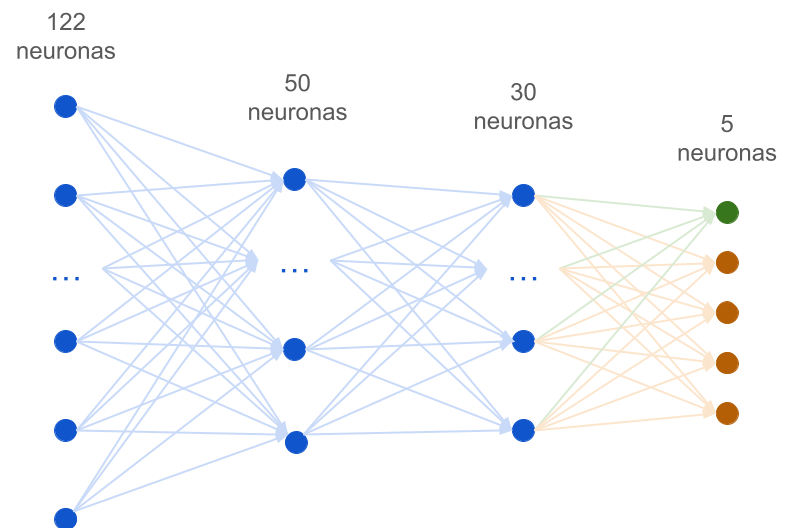
\includegraphics[width=0.4\textwidth]{img/kddDNN.png}
    \caption{Arquitectura de la Red Neuronal Profunda (DNN), donde el color verde hace referencia a que se clasifica como benigno y el color rojo como uno de los cuatro tipos de malware.}
    \label{fig:kddDNN}
\end{figure}

Una vez tenemos definida la arquitectura de nuestro modelo, es hora de elegir los hiperparámetros necesarios para entrenarlo. El optimizador elegido es Adam (\textit{Adaptive Moment Estimation}), configurado con una tasa de aprendizaje inicial de 0.001. Para la función de pérdida, se utilizó la entropía cruzada categórica (\lstinline|categorical_crossentropy|). Esta función es adecuada para problemas de clasificación multiclase, como nuestro problema con la base de datos \textit{KDD Cup 1999}. Aunque en el análisis que vamos a hacer posteriormente solo tenemos en cuenta si las instancias son malignas o benignas, se ha decidido hacer una clasificación multiclase ya que se obtiene mayor información y que además posteriormente se puede pasar a una clasificación binaria fácilmente. 

El modelo se entrenó durante 30 épocas, utilizando un tamaño de lote de 32 muestras por lote. Esta configuración permite un balance adecuado entre la velocidad de entrenamiento y la estabilidad de la convergencia. 

Además, he decidido añadir el \textit{callback} \lstinline|EarlyStopping| para detener el entrenamiento si la pérdida en el conjunto de validación no mejora después de 5 épocas, ayudando a prevenir el sobreajuste. Además, se emplea un \lstinline|CSVLogger| para registrar las métricas de entrenamiento y validación en cada época. La Figura~\ref{fig:kdd_dnn} presenta la evolución de la precisión y la pérdida a lo largo de las épocas de entrenamiento, destacando la mejora continua del modelo.

\begin{figure}[h]
    \centering
    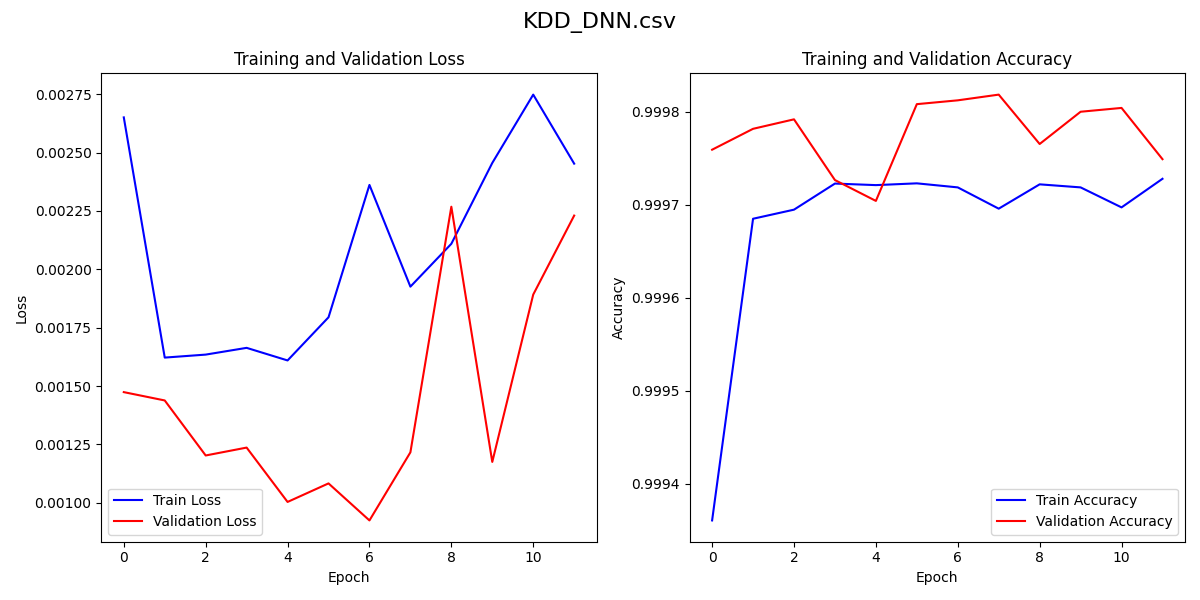
\includegraphics[width=0.6\textwidth]{img/KDD_DNN.csv.png}
    \caption{Evolución de la Precisión y la Pérdida durante el Entrenamiento del Modelo DNN.}
    \label{fig:kdd_dnn}
\end{figure}

En la imagen \ref{fig:kdd_dnn} se aprecian fluctuaciones en la pérdida de entrenamiento y validación a lo largo de todo el entrenamiento. La pérdida desciende hasta la época 6 y luego asciende. En cuanto a la precisión, se observa que es muy alta a lo largo de todo el entrenamiento, alrededor del 0.99. Aunque las curvas muestran fluctuaciones, estas son en realidad pequeñas variaciones en las centésimas del porcentaje. 

Podemos apreciar que, a pesar de que el número de épocas iniciales era de 30, no aparecen resultados a partir de la 11. Esto es debido a que en la época 6 el modelo ha obtenido un \lstinline|val_loss = 0,001| y desde esta época a la 11 no ha obtenido un valor menor, luego se ha producido la parada temprana, restaurando los pesos de la época 6. El valor del \textit{training loss} en esta época es de 0,00231. Por otra parte, la precisión de clasificación multiclase en esta época es de 0,997 en el entrenamiento y 0,998 en la validación. 


\subsection{Evaluación del modelo}

Después de entrenar el modelo, se evalúa como una clasificación binaria, usando el conjunto de datos que habíamos reservado para esta parte. Para empezar vamos a ver la matriz de confusión \ref{fig: dnnKDDConfusion} con el número de instancias que están bien clasificadas y mal clasificadas.

\begin{figure}[H]
    \centering
    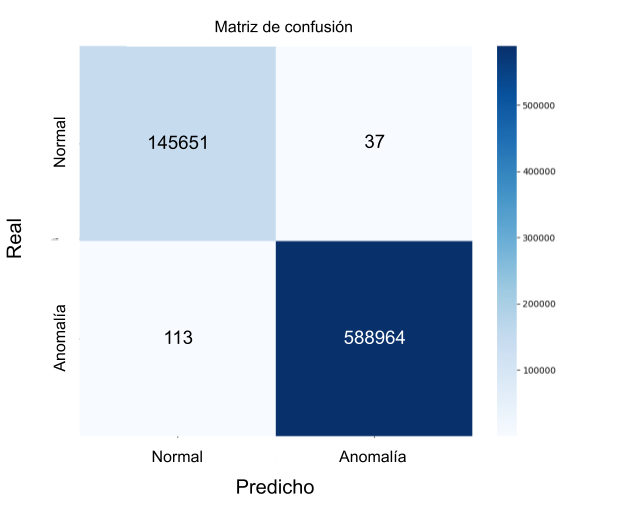
\includegraphics[width=0.4\textwidth]{img/confusionMatrixDNN_KDD.png}
    \caption{Matriz de confusión del modelo utilizando una DNN.}
    \label{fig: dnnKDDConfusion}
\end{figure}


En ella se puede observar como la mayoría de las predicciones están bien clasificadas ya que la mayoría de muestras se encuentran en la diagonal. Para poder ver con más detalle estos resultados, veamos ahora la tabla \ref{tab:kddDNN}, en la que podremos ver la precisión del modelo, su sensibilidad, la especificidad y el \textit{F1-Score}. Los resultados indican un desempeño sobresaliente en todas las métricas evaluadas, cada una con un valor de 0.999.

\begin{table}[H]
\centering
\begin{tabular}{|c|c|c|c|c|}
\hline
Modelo & Precisión & Sensibilidad & Especificidad & F1 Score \\ \hline
DNN & 0.999 & 0.999 & 0.999 & 0.999 \\ \hline
\end{tabular}
\caption{Métricas de rendimiento de la red neuronal profunda.}
\label{tab:kddDNN}
\end{table}

La precisión de 0.999 indica que el modelo clasifica correctamente prácticamente todos los registros de conexión. La especificidad de 0.999 muestra que el modelo detecta casi todos los registros anómalos, minimizando los falsos benignos. La sensibilidad de 0.999 revela que el modelo identifica correctamente casi todos los datos benignos. Finalmente, el \textit{F1-Score} obtiene un 0.999, lo que confirma gran capacidad del modelo para identificar correctamente tanto las instancias benignas como anómalas.










\section{Red Neuronal Recurrente}

Después de evaluar la red neuronal profunda, vamos a crear otro modelo predictivo para ver si podemos obtener unos resultados mejores. En este caso, vamos a enfocar el estudio en implementar una \acrfull{rnn} con \textit{Long Short-Term Memory} (RNN-LSTM) para este problema de detección de intrusiones. Se va a seguir principalmente las metodologías propuestas en \citep{yin2017deep,kim2016long}.

\subsection{Arquitectura del Modelo}

El modelo LSTM comienza con una capa de entrada que recibe los datos preprocesados anteriormente con una dimensión de 122 características. Estos datos son procesados por una capa LSTM que contiene 80 unidades ocultas. Este número de neuronas ha sido escogido después de obtener los mejores resultados comparado con otro números de neuronas ocultas en el artículo \citep{yin2017deep}. Esta capa LSTM es crucial ya que es capaz de capturar características a largo plazo en secuencias de datos, lo cual es esencial para nuestro estudio.

A continuación, la salida de la capa LSTM se pasa a una capa completamente conectada (capa Densa). Esta capa Densa tiene 5 neuronas, que corresponden a las 5 clases de salida. Se escoge 5 clases en vez de 2 porque creemos que este número de neuronas nos da más información y además nos da la posibilidad de hacer un análisis más extenso de sus resultados. La función de activación utilizada en esta capa es \textit{softmax}, la cual convierte los valores de salida en una distribución de probabilidad sobre las posibles clases, permitiendo así realizar la clasificación. Podemos ver un esquema de la arquitectura en la imagen \ref{fig:kddRNN}.

\begin{figure}[h]
    \centering
    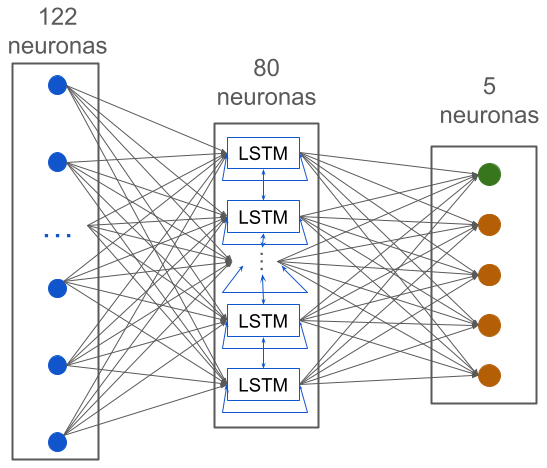
\includegraphics[width=0.4\textwidth]{img/kddRNN.png}
    \caption{Arquitectura de la Red Neuronal Recurrente (RNN), donde el color verde hace referencia a que se clasifica como benigno y el color rojo como uno de los cuatro tipos de malware.}
    \label{fig:kddRNN}
\end{figure}

Una vez definido el modelo, se procede a su compilación utilizando el optimizador \textit{Stochastic Gradient Descent} (SGD) con una tasa de aprendizaje que se va ajustando a lo largo del entrenamiento. Este optimizador se elige por su simplicidad y eficacia en muchos problemas de aprendizaje automático. Para la función de pérdida, se utilizó la entropía cruzada categórica (\lstinline|categorical_crossentropy|) como en el modelo anterior ya que tenemos 5 neuronas en la capa de salida.

El modelo se entrena durante 50 épocas con un tamaño de lote de 50. Al igual que en el modelo de DNN, he decidido añadir los \textit{callbacks} \lstinline|CSVLogger| y \lstinline|EarlyStopping| para registrar el proceso de entrenamiento y para prevenir el sobreajuste respectivamente. La Figura~\ref{fig:kdd_rnn} presenta la evolución de la precisión y la pérdida a lo largo de las épocas de entrenamiento.

\begin{figure}[h]
    \centering
    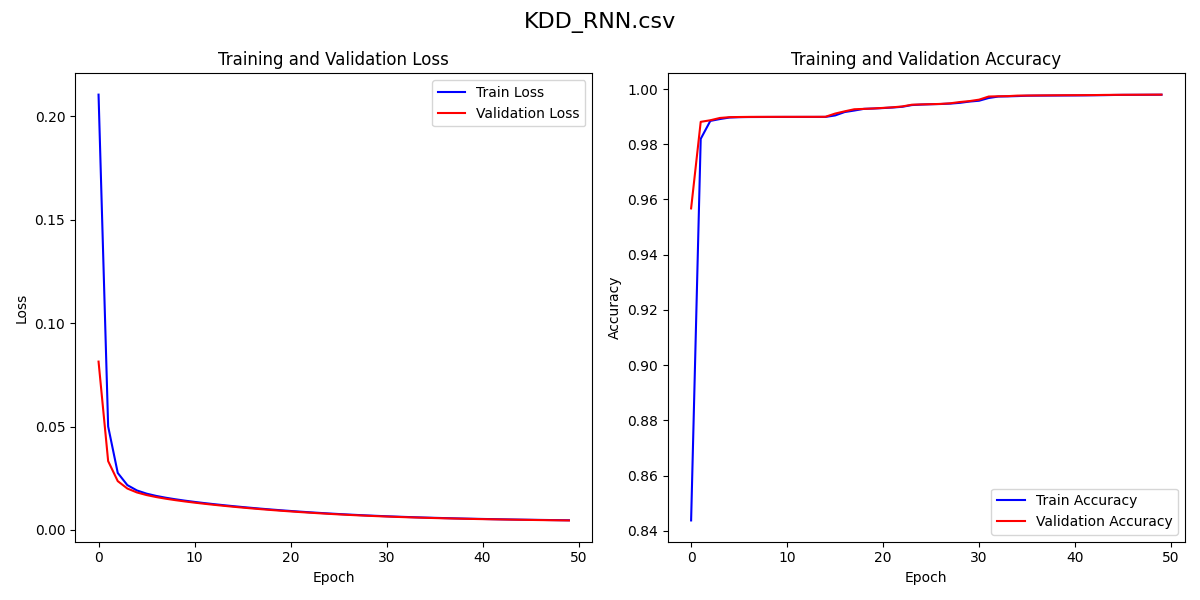
\includegraphics[width=0.55\textwidth]{img/KDD_RNN.csv.png}
    \caption{Evolución de la Precisión y la Pérdida durante el Entrenamiento del Modelo RNN - LSTM.}
    \label{fig:kdd_rnn}
\end{figure}

En la imagen \ref{fig:kdd_rnn}, observamos la evolución de la pérdida de entrenamiento y validación (gráfica izquierda). La pérdida de entrenamiento comienza alta, con un valor de 0.21, y disminuye rápidamente en las primeras 10 épocas. La pérdida de validación sigue un patrón similar, disminuyendo rápidamente y convergiendo con la pérdida de entrenamiento alrededor de la época 10. Ambas curvas se estabilizan alrededor de la época 20 y permanecen bajas, llegando a un valor de 0.004 para ambos subconjuntos. 

En la gráfica de la derecha, se observa la precisión de entrenamiento y validación. La precisión crece rápidamente en las primeras 10 épocas, para estabilizarse a partir de esa ápoca. Los datos de entrenamiento comienzan con un valor de 0.843, y aumenta rápidamente, alcanzando un valor de 0.999. La precisión de validación sigue de cerca a la precisión de entrenamiento, también alcanzando valores muy altos, 0.999. 

En ambas gráficas se observa un comportamiento muy parecido de ambas curvas, además de converger a unos resultados excelentes rápidamente, lo cual es un buen indicio de que el modelo está aprendiendo eficientemente y generalizando bien. 


\subsection{Evaluación del modelo}

Después de entrenar el modelo, se evalúa como una clasificación binaria, usando el conjunto de prueba que habíamos reservado anteriormente. Para empezar, vamos a ver la matriz de confusión \ref{fig: rnnKDDConfusion} con el número de registros de la \textit{KDD CUP 1999} que están bien clasificados y mal clasificados.

\begin{figure}[H]
    \centering
    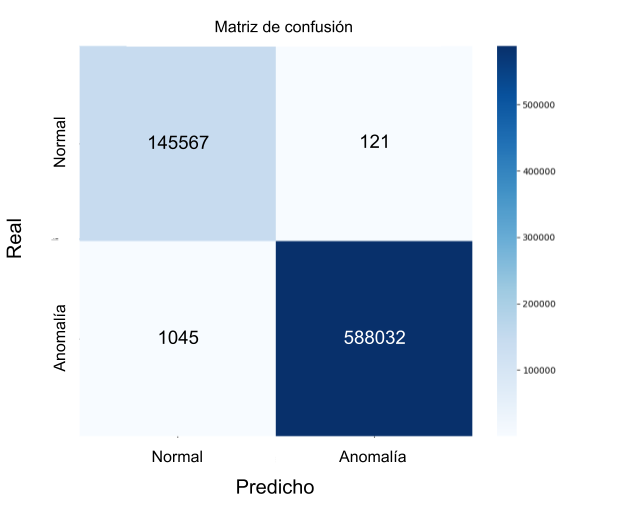
\includegraphics[width=0.4\textwidth]{img/confusionMatrixRNN_KDD.png}
    \caption{Matriz de confusión del modelo utilizando una RNN.}
    \label{fig: rnnKDDConfusion}
\end{figure}


En ella, al igual que en el modelo anterior (DNN), se puede observar como la mayoría de las predicciones se encuentran en la diagonal. Para poder ver con más detalle estos resultados, veamos ahora la tabla \ref{tab:kddRNN}, en la que podremos ver la precisión del modelo, su sensibilidad, la especificidad y el \textit{F1-Score}. Los resultados indican un desempeño sobresaliente en todas las métricas evaluadas, cada una con un valor de 0.999.

\begin{table}[H]
\centering
\begin{tabular}{|c|c|c|c|c|}
\hline
Modelo & Precisión & Sensibilidad & Especificidad & F1 Score \\ \hline
RNN & 0.998 & 0.999 & 0.998 & 0.998 \\ \hline
\end{tabular}
\caption{Métricas de rendimiento de la red neuronal recurrente.}
\label{tab:kddRNN}
\end{table}

En la tabla podemos volver a apreciar el gran rendimiento de este modelo con el conjunto de datos \textit{KDD CUP 1999}. Las métricas expuestas anteriormente nos muestran unos resultados excelentes, con valores prácticamente iguales a 1. Esto nos indica que la RNN - LSTM tiene una capacidad casi perfecta para distinguir entre registros anómalos y benignos. 












\section{Autoencoder}
A continuación, se plantea el problema de detección de intrusiones utilizando uno de los métodos más utilizados para resolver este problema, el \textit{autoencoder} \citep{podder2021artificial}. La estrategia consiste en entrenar el \textit{autoencoder} exclusivamente con un subconjunto de datos benignos. Posteriormente, se evalúa la capacidad del modelo para reconstruir los demás registros. En función del error de reconstrucción, los registros se clasificarán como normales o como malware, basándose en un umbral predefinido. Este enfoque se basa principalmente en el trabajo de \citep{xu2021improving}.


\subsection{Arquitectura del modelo}

El \textit{autoencoder} propuesto para esta sección contiene 5 capas densas en las que se codifica una representación de características de 122 dimensiones en un vector de 5 dimensiones en su capa latente. Antes de llegar a esta dimensión, primero se reduce de 122 a 32 para a continuación reducir aun más hasta llegar a 5. Después, este representación comprimida de los datos se decodifican de vuelta a un vector de 32 dimensiones y después a 122 como los datos de entrda. En la imagen \ref{fig:architectureAE} podemos ver de manera más gráfica su arquitectura.

\begin{figure}[H]
    \centering
    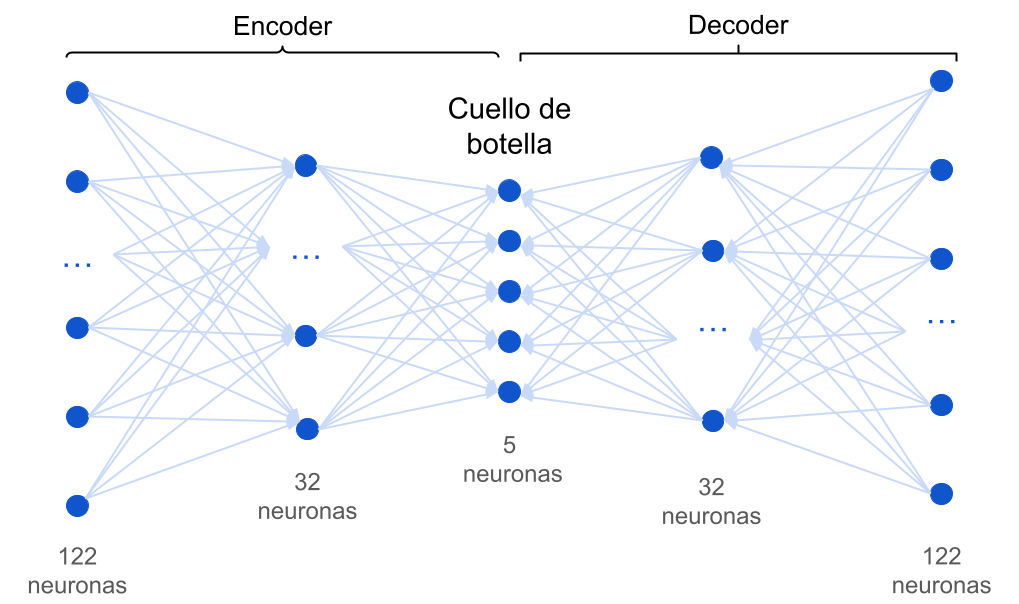
\includegraphics[width=0.4\textwidth]{img/kddAE.png} 
    \caption{Arquitectura del \textit{autoencoder} con 5 capas densas.}
    \label{fig:architectureAE}
\end{figure}

Las capas ocultas son capas densas, es decir, están completamente conectadas y utilizan como función de activación ReLU. El error de reconstrucción entre la entrada $x$ y la salida reconstruida $\hat{x}$ se calcula usando el error absoluto medio (MAE).

Una vez definido el modelo, se procede a compilarlo utilizando el optimizador Adam con un \textit{learning rate} inicial de 0,001. 

\begin{minipage}{0.6\textwidth}
    El modelo se entrena durante 30 épocas en mini lotes de 30 registros. Al igual que en los dos modelos anteriores, he decidido añadir los \textit{callbacks} \lstinline|CSVLogger| y \lstinline|EarlyStopping| para registrar el proceso de entrenamiento y para prevenir el sobreajuste respectivamente. La Figura~\ref{fig:trainingAE} presenta la evolución de la precisión y la pérdida a lo largo de las épocas de entrenamiento.

    \bigskip

    En la figura, se observa la evolución de la pérdida de entrenamiento y validación a lo largo de las 30 épocas. Al inicio del entrenamiento, se aprecia un descenso rápido en ambas curvas de pérdida. Esto indica que el modelo está aprendiendo eficazmente las características de los datos durante las primeras épocas, lo que es un buen signo de que la fase inicial del entrenamiento está ajustando bien los pesos.
\end{minipage}
\begin{minipage}{0.05\textwidth}
    \textbf{ }
\end{minipage}
\begin{minipage}{0.33\textwidth}
    
    \begin{figure}[H]
    \centering
    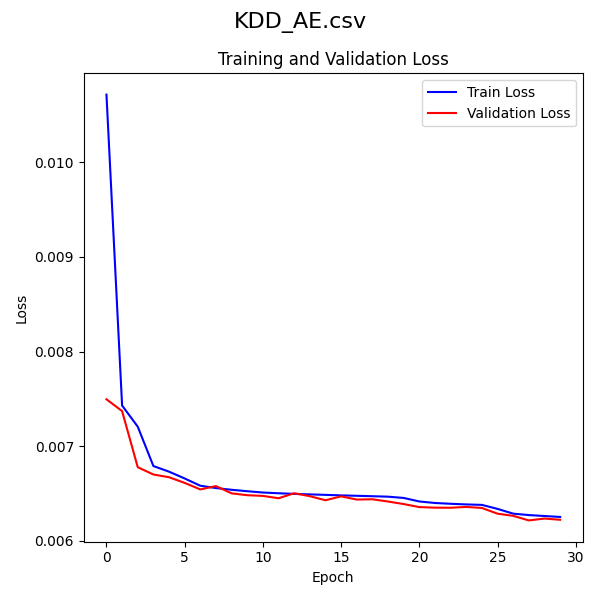
\includegraphics[width=\textwidth]{img/KDD_AE.csv.png}
    \captionof{figure}{Evolución de la pérdida durante el entrenamiento del \textit{autoencoder}}
    \label{fig:trainingAE}
    \end{figure}

\end{minipage}


A partir de la época 15, tanto la pérdida de entrenamiento como la de validación comienzan a estabilizarse y converger alrededor de un valor constante 0,0064. Este comportamiento sugiere que el modelo ha alcanzado un punto de equilibrio donde las actualizaciones de los pesos no producen mejoras significativas, indicando una buena adaptación del modelo a los datos. Es importante destacar que a pesar de la buena adaptación del modelo a los datos de entrenamiento, ambas curvas son muy similares a lo largo de todas las épocas, lo que indica que el modelo generaliza bien los datos de entrenamiento sin llegar al sobreajuste.


\subsection{Evaluación del modelo}


Después de entrenar el modelo con los datos normales de entrenamiento, se procede a la evaluación del modelo. Para ello, primero tenemos que fijar un umbral que nos diga si un registro es malware o normal dependiendo de su error de reconstrucción. Para ello, utilizando la función de \lstinline|sklearn.metrics|, \lstinline|precision_recall_curve|, se calcula la curva de precisión y recuperación (\textit{Precision-Recall}) en función de diferentes umbrales que se utilicen para clasificar los registros. A partir de esta curva, se selecciona un umbral alto que balancee la precisión y la recuperación para la detección de anomalías. Este proceso se ilustra en la siguiente gráfica:

\begin{figure}[H]
    \centering
    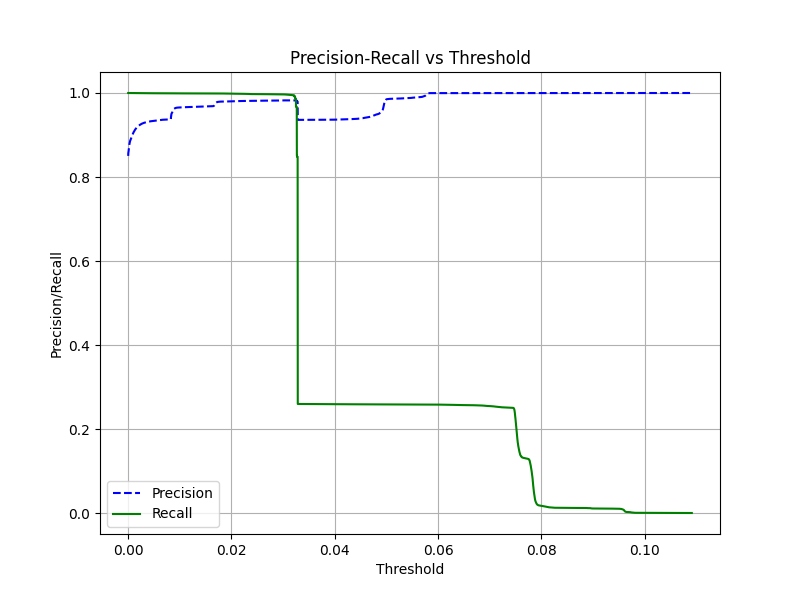
\includegraphics[width=0.4\textwidth]{img/umbral.png} 
    \caption{Gráfica de precisión y recuperación en función del umbral}
    \label{fig:precision_recall}
\end{figure}

Nuestro objetivo consiste en minimizar los registros anómalos que se clasifiquen como normales. Para ello, tenemos que encontrar un umbral que maximice el \textit{recall}. Un valor que maximiza tanto el recall como la precisión es 0.02, luego se decide utilizar este valor como umbral. 

Con este umbral, vamos a evaluar el modelo usando los datos de prueba. Para empezar, vamos a ver la matriz de confusión \ref{fig: aeKDDConfusion} con el número de registros de la \textit{KDD CUP 1999} que están bien clasificados y mal clasificados.

\begin{figure}[H]
    \centering
    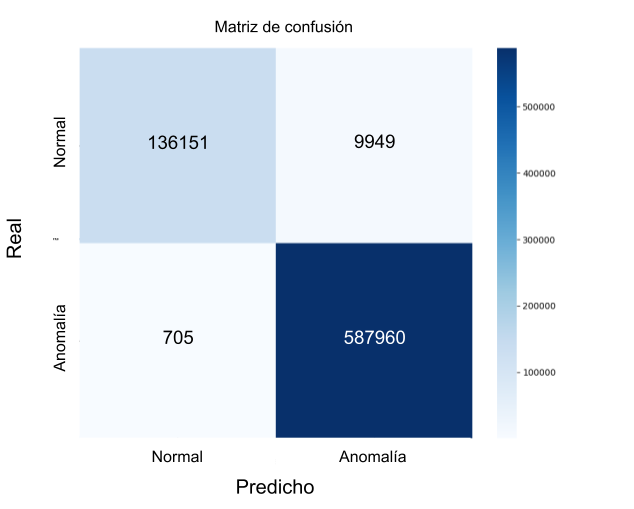
\includegraphics[width=0.4\textwidth]{img/confusionMatrixAE_KDD.png}
    \caption{Matriz de confusión del modelo utilizando una \textit{autoencoder}.}
    \label{fig: aeKDDConfusion}
\end{figure}


En ella, al igual que en los otros dos modelos, se obtienen unos resultados excelentes. Veamos ahora la tabla \ref{tab:kddAE} con el resto de métricas.
\begin{table}[H]
\centering
\begin{tabular}{|c|c|c|c|c|}
\hline
Modelo & Precisión & Sensibilidad & Especificidad & F1 Score \\ \hline
Autoencoder & 0.999 & 0.93 & 0.999 & 0.991 \\ \hline
\end{tabular}
\caption{Métricas de rendimiento del \textit{autoencoder}.}
\label{tab:kddAE}
\end{table}

En la tabla podemos volver a apreciar el gran rendimiento de este modelo con el conjunto de datos \textit{KDD CUP 1999}. Las métricas expuestas anteriormente nos muestran unos resultados excelentes, con valores prácticamente iguales a 1. Estos nos indica que la arquitectura de \textit{autoencoder} utilizada tiene una capacidad casi perfecta para detectar tanto registros benignos como registros anómalos. 






\section{Red Neuronal Convolucional}

Por último, vamos a plantear el problema de detección de intrusiones utilizando una CNN. Este problema no estaba clasificado en el \textit{review} \citep{podder2021artificial}, pero con el conocimiento que ya poseíamos sobre este método unido a la búsqueda de un artículo que tratara este tema, hemos decidido optar por hacer un estudio con esta red neuronal. Para ello, se va a seguir la metodología que se usa en \citep{kim2020cnn, yao2021intrusion}.

\subsection{Visualización de los datos}

En la subsección \ref{sec:datoskdd} estudiamos como procesar los datos originales de la base de datos, a datos que pudieran ser utilizados por la redes neuronales. Pasamos de un vector de 41 características con diferentes tipos de datos, a un vector de 122 características donde todos los elementos eran números reales entre 0 y 1. Como bien hemos visto en el capítulo \ref{Capitulo_2}, las CNN son redes neuronales que están diseñadas para procesar datos almacenados en matrices. En este caso, al igual que en el modelo de CNN utilizado en la clasificación de malware, vamos a pasar del vector unidimensional a un vector bidimensional. 

En el artículo \citep{kim2020cnn}, los datos son más antiguos que los actuales y en vez de tener un vector de 122 dimensiones, ellos tienen un vector de 117 dimensiones que redimensionan a una matriz $13 \times 9$. En el artículo \citep{yao2021intrusion}, pasan del vector de 41 características a una matriz $7 \times 7$ y los valores restantes le asignan un 0. En nuestro caso, he decido hacer un estudio más exhaustivo de las 122 características para ver que opciones podía plantear para convertir el vector en matriz.

Primero se observó que $122 = 61 \times 2$. Creí que esta matriz no sería muy efectiva de primera mano, ya que había una gran diferencia entre el número de filas y el número de columnas. En este punto, decidí hacer un estudio de las 122 características. Como para estandarizar los datos tuve que calcular los máximos y mínimos de cada característica, decidí fijarme en ellos. Se me ocurrió ver si había alguna característica que siempre valiera lo mismo. Esto era tan fácil como comprobar si algún valor máximo era igual a su valor mínimo. Sea $D_i$ el conjunto de todas las características $i$-ésimas del \textit{dataset}, entonces, 
\begin{equation}
    \exists i \in [1,122] \hspace{2mm} _{\shortparallel} \hspace{2mm} \forall x \in D_i \hspace{2mm} _{\shortparallel} \hspace{2mm} \min(D_i) \leq x \leq \max(D_i) = \min(D_i)
\end{equation}
luego $\forall x \in D_i, x = \min(D_i)$. Comprobando esta propiedad, me dí cuenta que la característica 101 siempre valía 0, es decir la característica 20 de los datos originales (las instrucciones salientes en FTP, que se refiere al número de comandos enviados desde el servidor FTP hacia un cliente durante una sesión de transferencia de archivos). Entonces, he decidido prescindir de esta característica para pasar de un vector de 122 dimensiones a un vector de 121 dimensiones que puede redimensionarse a una matriz $11 \times 11$. 

\begin{figure}[H]
    \centering
    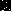
\includegraphics[width=0.2\textwidth]{img/descarga.png}
    \caption{Visualización de un registro benigno del \textit{KDD CUP 1999}.}
    \label{fig: kddimage}
\end{figure}


\subsection{Arquitectura del Modelo}

La arquitectura del modelo CNN se compone de varias capas convolucionales, de \textit{max-pooling} y densas, diseñadas para procesar las matrices \(11 \times 11\) generadas en la fase de preprocesamiento. La primera capa convolucional aplica 64 filtros convolucionales con un tamaño de kernel de \(3 \times 3\), utilizando la función de activación ReLU. Esta capa inicial se encarga de detectar las características locales más importantes de la imagen. 

A continuación, se utiliza una capa de Max-Pooling con un tamaño de ventana de \(2 \times 2\) para reducir la dimensionalidad de los mapas de características, conservando la información relevante y disminuyendo la carga computacional.

La segunda capa convolucional aplica 128 filtros convolucionales con un tamaño de kernel de \(3 \times 3\), también con función de activación ReLU. Esta capa permite capturar características más complejas a un nivel superior de abstracción, detectando patrones más detallados en los datos.

Después de la segunda capa convolucional, se emplea otra capa de \textit{max-pooling} con un tamaño de ventana de \(2 \times 2\), para continuar reduciendo la dimensionalidad de los mapas de características y conservar los patrones más importantes.

Los mapas de características obtenidos se aplanan y pasan a través de una capa densa de 128 neuronas con función de activación ReLU. Esta capa permite compactar la información obtenida por las capas convolucionales. Después, se pasa la información por una capa dens con 64 neuronas y función de activación ReLU refina aún más esta representación. 

Finalmente, se pasa por la capa de salida con la función de activación softmax, que es una capa densa con 5 neuronas como en la RNN y la DNN, ya que de esta forma se obtiene más información aunque luego se haga un análisis de clasificación binaria.

\begin{figure}[h]
    \centering
    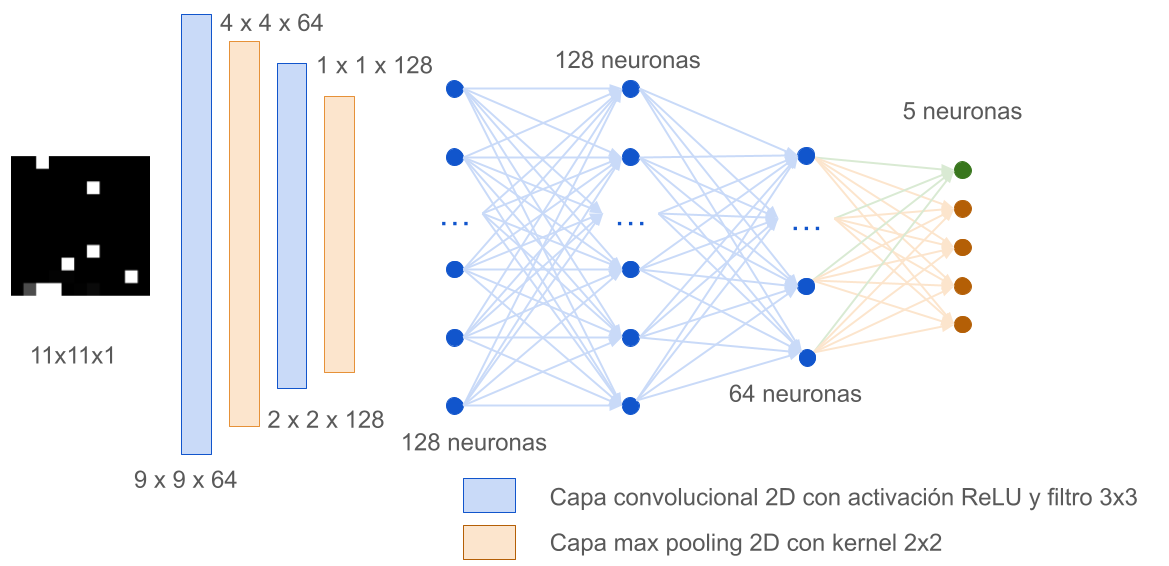
\includegraphics[width=0.7\textwidth]{img/kddCNN.png}
    \caption{Arquitectura de la Red Neuronal Convolucional para la detección de intrusiones de la \textit{KDD CUP}.}
    \label{fig:kdd_cnn_architecture}
\end{figure}


Una vez creada la arquitectura de la CNN, se compila el modelo con el optimizador Adam con una tasa de aprendizaje inicial de 0,001. La función de pérdida seleccionada es \lstinline|categorical_crossentropy|. El modelo se entrena en lotes de tamaño 32 durante 30 época. 

Como en los modelos anteriores, se añaden los \textit{callbacks} \lstinline|EarlyStopping| y \lstinline|CSVLogger| para evitar el sobreajuste y registrar las métricas de entrenamiento respectivamente. La evolución del entrenamiento a lo largo de las 30 épocas se puede ver en la imagen \ref{fig:cnn_training_process}.

\begin{figure}[h]
    \centering
    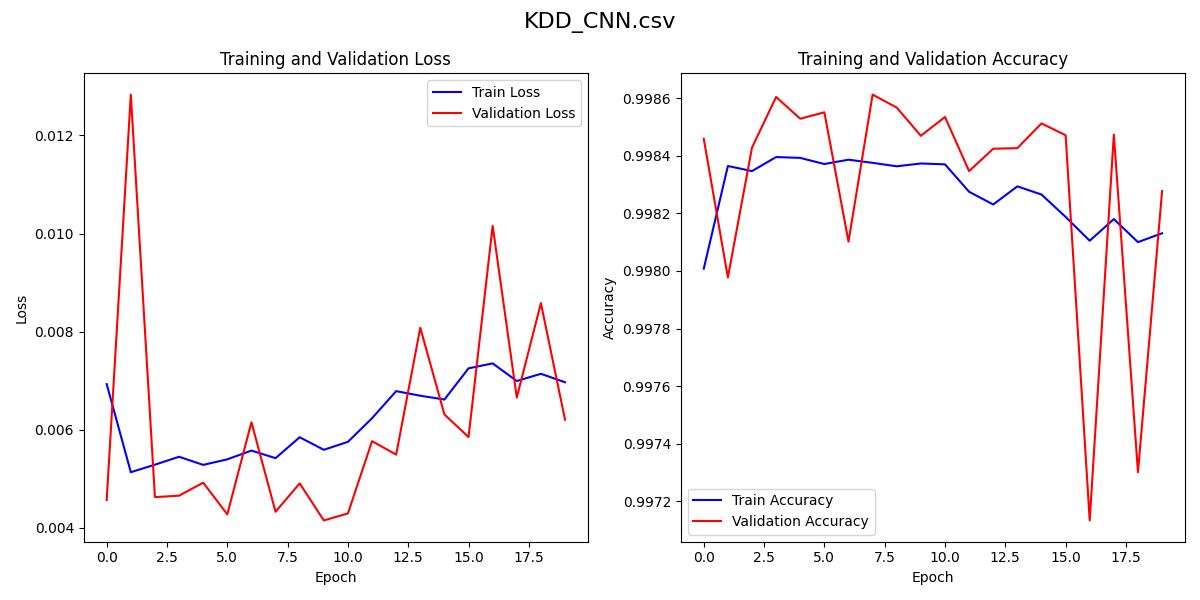
\includegraphics[width=0.5\textwidth]{img/KDD_CNN.csv.png}
    \caption{Evolución de la precisión y la pérdida durante el entrenamiento de la CNN.}
    \label{fig:cnn_training_process}
\end{figure}


En la imagen, podemos observar la evolución de la pérdida de entrenamiento y validación (gráfica izquierda). La pérdida de entrenamiento comienza en un valor bajo, 0.006, y muestra fluctuaciones a lo largo de las épocas, sin una tendencia clara de descenso o ascenso. Es importante notar que estas fluctuaciones son de centésimas, lo que implica que son casi mínimas. La pérdida de validación muestra grandes picos y valles, especialmente al inicio, lo cual indica una inestabilidad en la capacidad del modelo para generalizar en diferentes épocas.

En la gráfica de la derecha, se observa la precisión de entrenamiento y validación. La precisión de entrenamiento comienza en un valor alto, 0.9972, y muestra fluctuaciones a lo largo de las épocas, similar a la pérdida. Nuevamente, estas fluctuaciones son de centésimas, indicando variaciones mínimas. La precisión de validación muestra un patrón muy variable, con grandes picos y valles, reflejando la inestabilidad observada en la pérdida.

Como se puede observar en la gráfica, a pesar de que el entrenamiento estaba previsto para 30 épocas, se ha detenido en la vuelta 19. Esto es porque en la época 9 se obtiene el menor \lstinline|val_loss = 0.0041|. Además, en esta época, la pérdida de entrenamiento es \lstinline|loss = 0.0056|, la precisión de validación es \lstinline|val_accuracy = 0.998| y la precisión de entrenamiento vale \lstinline|accuracy = 0.998|. Esto sugiere que, a pesar de las fluctuaciones observadas, el modelo alcanzó un rendimiento óptimo en esta época.


\subsection{Evaluación del modelo}


Después de entrenar el modelo, se evalúa como una clasificación binaria, usando el 15\% del conjunto de datos reservado para esta parte. Para empezar, vamos a ver la matriz de confusión \ref{fig: cnnKDDConfusion} con el número de registros de la \textit{KDD CUP 1999} que están bien clasificados y mal clasificados.

\begin{figure}[H]
    \centering
    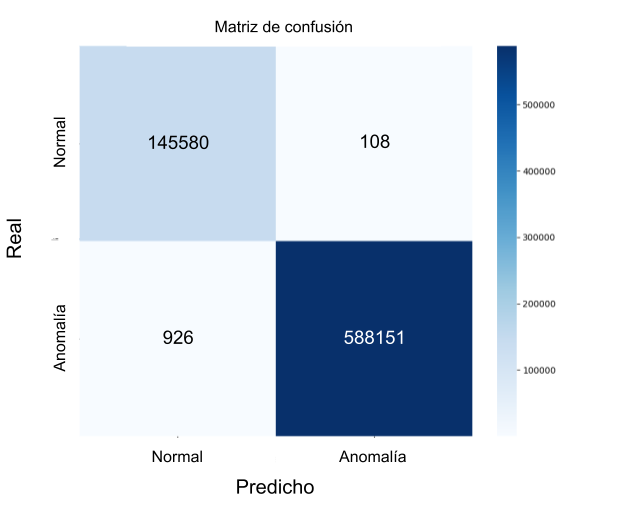
\includegraphics[width=0.4\textwidth]{img/confusionMatrixCNN_KDD.png}
    \caption{Matriz de confusión del modelo utilizando una CNN.}
    \label{fig: cnnKDDConfusion}
\end{figure}


En ella, al igual que en los 3 modelos anteriores, se obtienen unos resultados excelentes. Veamos ahora la tabla \ref{tab:kddCNN} con el resto de métricas.
\begin{table}[H]
\centering
\begin{tabular}{|c|c|c|c|c|}
\hline
Modelo & Precisión & Sensibilidad & Especificidad & F1 Score \\ \hline
CNN & 0.999 & 0.999 & 0.998 & 0.998 \\ \hline
\end{tabular}
\caption{Métricas de rendimiento de la red neuronal convolucional.}
\label{tab:kddCNN}
\end{table}

En la tabla podemos volver a apreciar el gran rendimiento de este modelo con el conjunto de datos \textit{KDD CUP 1999}. Las métricas expuestas anteriormente nos muestran unos resultados excelentes, con valores prácticamente iguales a 1. Estos nos indica que la arquitectura de CNN utilizada tiene una capacidad casi perfecta para detectar tanto registros benignos como registros anómalos. 







\section{Resultados}


En este estudio, se han implementado y evaluado cuatro modelos de redes neuronales diferentes para la detección de intrusiones utilizando el conjunto de datos \textit{KDD Cup 1999}. Los modelos considerados fueron una \acrfull{dnn}, una \acrfull{rnn}, un \textit{autoencoder} y una \acrfull{cnn}. A continuación, se resumen los resultados obtenidos por cada uno de estos modelos.

El modelo DNN mostró un rendimiento sobresaliente con una precisión, sensibilidad, especificidad y \textit{F1-Score} de 0.999 en la clasificación binaria de registros benignos y anómalos. Aunque las fluctuaciones en las curvas de pérdida y precisión indicaron pequeñas variaciones, el modelo logró una excelente generalización. Los resultados detallados se presentan en la Tabla~\ref{tab:conclusionModels}.

El modelo RNN-LSTM también obtuvo un rendimiento notable, con métricas de rendimiento casi perfectas, similar al DNN. La precisión y la pérdida se estabilizaron rápidamente, alcanzando valores de 0.999 en las métricas evaluadas. Las curvas de precisión y pérdida mostraron la mejor estabilidad, inclinándose de manera constante sin fluctuaciones notables, lo que indica una excelente capacidad de aprendizaje y generalización de las características temporales de los datos. Los resultados se detallan en la Tabla~\ref{tab:conclusionModels}.

El \textit{autoencoder} mostró un rendimiento excelente en la detección de intrusiones, con una precisión de 0.999 y un \textit{F1-Score} de 0.991. Aunque su sensibilidad fue ligeramente inferior (0.93), su capacidad para reconstruir los registros benignos y detectar anomalías fue altamente efectiva. El umbral de 0.02 se utilizó para clasificar los registros, maximizando tanto la precisión como el \textit{recall}. Los resultados se presentan en la Tabla~\ref{tab:conclusionModels}.

Por último, la CNN también obtuvo resultados excelentes, con métricas de rendimiento cercanas a 1. Al transformar los vectores de características en matrices $11 \times 11$, el modelo pudo aprender eficazmente las características espaciales de los datos. Los resultados indicaron una gran capacidad para detectar tanto registros benignos como anómalos, con valores muy altos en todas las métricas evaluadas, a pesar de sufrir fluctuaciones a lo largo de todo el entrenamiento (tabla \ref{tab:conclusionModels}).

Aunque todos los modelos obtuvieron resultados excelentes en la detección de intrusiones, el modelo RNN-LSTM destacó por su capacidad de aprender y generalizar eficientemente las características temporales de los datos. Su rendimiento consistente a lo largo de las épocas, junto con sus resultados en las métricas de precisión, sensibilidad, especificidad y \textit{F1-Score}, lo convierten en el mejor modelo entre los evaluados. Por lo tanto, se concluye que la RNN-LSTM es la opción más efectiva para la detección de intrusiones en el conjunto de datos \textit{KDD Cup 1999}, proporcionando resultados sobresalientes y un rendimiento superior en comparación con los otros modelos.

\begin{table}[H]
\centering
\begin{tabular}{|l|c|c|c|c|}
\hline
\textbf{Modelo} & \textbf{Precisión} & \textbf{Sensibilidad} & \textbf{Especificidad} & \textbf{F1 Score} \\ \hline
DNN & 0.999 & 0.999 & 0.999 & 0.999 \\ \hline
RNN & 0.998 & 0.999 & 0.998 & 0.998 \\ \hline
Autoencoder & 0.999 & 0.93 & 0.999 & 0.991 \\ \hline
CNN & 0.999 & 0.998 & 0.999 & 0.999 \\ \hline
\end{tabular}
\caption{Métricas de rendimiento de los diferentes modelos.}
\label{tab:conclusionModels}
\end{table}






\begin{comment}
Improving Performance of Autoencoder-Based
Network Anomaly Detection on NSL-KDD Dataset

Malware traffic classification using convolutional neural network for representation learning

Deep Learning-based Feature Selection for Intrusion Detection
System in Transport Layer 1)


    Para implementar el proceso descrito, puedes usar un Autoencoder (AE), que es un tipo de red neuronal utilizada para aprender representaciones eficientes (codificaciones) de datos, típicamente para la reducción de dimensionalidad.

Explicación del Proceso:
Fase de Entrenamiento:

Extracción y Reducción de Características: Las características originales del tráfico de red se extraen y se reducen mediante la operación de codificación del Autoencoder. Esto significa que los datos se pasan a través de la parte de codificación del AE para obtener una representación en un espacio latente.
Reconstrucción del Tráfico: El espacio latente se usa para reconstruir la salida (decodificación).
Cálculo del Error de Reconstrucción: La diferencia entre la muestra de tráfico original y la reconstruida se calcula para obtener el error de reconstrucción.
Determinación del Umbral: Se calcula el valor máximo de todos los errores de reconstrucción como el umbral para identificar anomalías.
Fase de Prueba:

Cálculo del Error de Reconstrucción: Las muestras de tráfico de red se ingresan al modelo AE entrenado y se calcula el error de reconstrucción, ahora llamado "puntaje de anomalía".
Comparación con el Umbral: Si el puntaje de anomalía es mayor que el umbral determinado durante la fase de entrenamiento, la muestra de tráfico se considera anómala.
Código en Python
Aquí tienes un ejemplo de cómo implementar este proceso en Python utilizando Keras y TensorFlow:

python
Copiar código
import numpy as np
from tensorflow.keras.models import Model
from tensorflow.keras.layers import Input, Dense
from tensorflow.keras import backend as K

# Fase de Entrenamiento
def crear_autoencoder(input_dim, encoding_dim):
    # Definición del Autoencoder
    input_layer = Input(shape=(input_dim,))
    encoder = Dense(encoding_dim, activation="relu")(input_layer)
    decoder = Dense(input_dim, activation="sigmoid")(encoder)
    autoencoder = Model(inputs=input_layer, outputs=decoder)
    autoencoder.compile(optimizer="adam", loss="mean_squared_error")
    return autoencoder

def entrenar_autoencoder(autoencoder, datos):
    # Entrenar el Autoencoder
    autoencoder.fit(datos, datos, epochs=50, batch_size=256, shuffle=True, validation_split=0.2)
    return autoencoder

def calcular_umbral(autoencoder, datos):
    # Calcular errores de reconstrucción
    reconstrucciones = autoencoder.predict(datos)
    errores = np.mean(np.power(datos - reconstrucciones, 2), axis=1)
    umbral = np.max(errores)
    return umbral

# Fase de Prueba
def detectar_anomalias(autoencoder, datos, umbral):
    # Calcular errores de reconstrucción
    reconstrucciones = autoencoder.predict(datos)
    errores = np.mean(np.power(datos - reconstrucciones, 2), axis=1)
    anomalias = errores > umbral
    return anomalias, errores

# Ejemplo de uso
input_dim = 30  # Supongamos que tenemos 30 características de tráfico de red
encoding_dim = 14  # Dimensión del espacio latente
datos_entrenamiento = np.random.rand(10000, input_dim)  # Datos de entrenamiento (ejemplo)

# Crear y entrenar el Autoencoder
autoencoder = crear_autoencoder(input_dim, encoding_dim)
autoencoder = entrenar_autoencoder(autoencoder, datos_entrenamiento)

# Calcular el umbral de errores de reconstrucción
umbral = calcular_umbral(autoencoder, datos_entrenamiento)

# Datos de prueba
datos_prueba = np.random.rand(1000, input_dim)

# Detectar anomalías en los datos de prueba
anomalias, puntajes_anomalia = detectar_anomalias(autoencoder, datos_prueba, umbral)

print("Umbral:", umbral)
print("Anomalías detectadas:", np.sum(anomalias))
Explicación del Código:
Crear el Autoencoder:

Definimos la arquitectura del Autoencoder con una capa de entrada, una capa de codificación y una capa de decodificación.
Entrenar el Autoencoder:

Entrenamos el Autoencoder utilizando los datos de entrenamiento. Aquí usamos un conjunto de datos de ejemplo generado aleatoriamente.
Calcular el Umbral:

Después de entrenar el Autoencoder, calculamos los errores de reconstrucción en los datos de entrenamiento y tomamos el valor máximo de estos errores como el umbral para la detección de anomalías.
Detectar Anomalías:

En la fase de prueba, calculamos los errores de reconstrucción para las nuevas muestras de tráfico de red y los comparamos con el umbral. Si el error de reconstrucción de una muestra es mayor que el umbral, se considera anómala.
Este enfoque proporciona un marco básico para la detección de anomalías en el tráfico de red utilizando un Autoencoder. Puedes ajustar los hiperparámetros, como el tamaño del espacio latente y el número de épocas, según tus necesidades y la naturaleza de tus datos.

entrenamos las muestras benignas o malignas?
ChatGPT
En el contexto de la detección de anomalías utilizando un Autoencoder (AE), generalmente entrenas el modelo con muestras benignas (normales). La idea es que el Autoencoder aprende a reconstruir bien las muestras normales, pero tendrá un mayor error de reconstrucción para las muestras anómalas (malignas) que no ha visto durante el entrenamiento.

Razones para Entrenar con Muestras Benignas:
Generalización: El Autoencoder se entrena para capturar la estructura de las muestras benignas. Las anomalías, al no seguir esta estructura, resultarán en mayores errores de reconstrucción.
Detección Eficaz de Anomalías: Un mayor error de reconstrucción sugiere que la muestra es diferente de lo que el modelo ha aprendido como normal, lo cual es indicativo de una anomalía.
Escasez de Datos Anómalos: En muchos casos, las muestras anómalas son escasas y pueden no estar disponibles en cantidad suficiente para un entrenamiento robusto.
Modificación del Código para Asegurarse de Entrenar Solo con Muestras Benignas
Aquí se asume que datos_entrenamiento contiene solo muestras benignas.

python
Copiar código
import numpy as np
from tensorflow.keras.models import Model
from tensorflow.keras.layers import Input, Dense

# Funciones para crear y entrenar el Autoencoder
def crear_autoencoder(input_dim, encoding_dim):
    input_layer = Input(shape=(input_dim,))
    encoder = Dense(encoding_dim, activation="relu")(input_layer)
    decoder = Dense(input_dim, activation="sigmoid")(encoder)
    autoencoder = Model(inputs=input_layer, outputs=decoder)
    autoencoder.compile(optimizer="adam", loss="mean_squared_error")
    return autoencoder

def entrenar_autoencoder(autoencoder, datos_benignos):
    autoencoder.fit(datos_benignos, datos_benignos, epochs=50, batch_size=256, shuffle=True, validation_split=0.2)
    return autoencoder

def calcular_umbral(autoencoder, datos_benignos):
    reconstrucciones = autoencoder.predict(datos_benignos)
    errores = np.mean(np.power(datos_benignos - reconstrucciones, 2), axis=1)
    umbral = np.max(errores)
    return umbral

# Función para detectar anomalías
def detectar_anomalias(autoencoder, datos, umbral):
    reconstrucciones = autoencoder.predict(datos)
    errores = np.mean(np.power(datos - reconstrucciones, 2), axis=1)
    anomalias = errores > umbral
    return anomalias, errores

# Ejemplo de uso
input_dim = 30  # Número de características de tráfico de red
encoding_dim = 14  # Dimensión del espacio latente

# Datos de entrenamiento (muestras benignas)
datos_entrenamiento_benignos = np.random.rand(10000, input_dim)  # Reemplaza esto con tus datos reales

# Crear y entrenar el Autoencoder con muestras benignas
autoencoder = crear_autoencoder(input_dim, encoding_dim)
autoencoder = entrenar_autoencoder(autoencoder, datos_entrenamiento_benignos)

# Calcular el umbral de errores de reconstrucción
umbral = calcular_umbral(autoencoder, datos_entrenamiento_benignos)

# Datos de prueba (pueden contener tanto benignos como malignos)
datos_prueba = np.random.rand(1000, input_dim)  # Reemplaza esto con tus datos reales

# Detectar anomalías en los datos de prueba
anomalias, puntajes_anomalia = detectar_anomalias(autoencoder, datos_prueba, umbral)

print("Umbral:", umbral)
print("Anomalías detectadas:", np.sum(anomalias))
Pasos en el Código:
Entrenamiento del Autoencoder con Muestras Benignas:

Asegúrate de que datos_entrenamiento_benignos contenga solo muestras de tráfico de red benignas.
El Autoencoder se entrena para reconstruir estas muestras benignas.
Cálculo del Umbral:

Calcula los errores de reconstrucción en las muestras benignas y establece el umbral como el valor máximo de estos errores.
Detección de Anomalías:

En la fase de prueba, cualquier muestra cuyo error de reconstrucción sea mayor que el umbral se considera anómala.
De esta manera, entrenar solo con muestras benignas permite al Autoencoder detectar efectivamente las anomalías basándose en la desviación de las características normales aprendidas.

como calcular el umbral?
ChatGPT
Calcular el umbral en el contexto de un Autoencoder (AE) para la detección de anomalías implica determinar un valor de referencia que diferencie entre las muestras normales y anómalas. El proceso es el siguiente:

Entrenar el Autoencoder con Muestras Benignas:

Entrena el AE solo con datos benignos (normales).
Calcular los Errores de Reconstrucción en los Datos de Entrenamiento:

Después del entrenamiento, pasa las mismas muestras benignas a través del AE para obtener las reconstrucciones.
Calcula el error de reconstrucción para cada muestra. Un error de reconstrucción comúnmente usado es el error cuadrático medio (MSE).
Determinar el Umbral:

Utiliza las estadísticas de los errores de reconstrucción para determinar un umbral. Una estrategia común es utilizar el valor máximo del error de reconstrucción de las muestras benignas, pero otras estrategias incluyen usar un percentil alto (por ejemplo, 95%) para tener una tolerancia a ciertos errores benignos.
Aquí tienes un código que muestra este proceso:

python
Copiar código
import numpy as np
from tensorflow.keras.models import Model
from tensorflow.keras.layers import Input, Dense
from sklearn.model_selection import train_test_split

# Función para crear el Autoencoder
def crear_autoencoder(input_dim, encoding_dim):
    input_layer = Input(shape=(input_dim,))
    encoder = Dense(encoding_dim, activation="relu")(input_layer)
    decoder = Dense(input_dim, activation="sigmoid")(encoder)
    autoencoder = Model(inputs=input_layer, outputs=decoder)
    autoencoder.compile(optimizer="adam", loss="mean_squared_error")
    return autoencoder

# Función para entrenar el Autoencoder
def entrenar_autoencoder(autoencoder, datos_benignos):
    autoencoder.fit(datos_benignos, datos_benignos, epochs=50, batch_size=256, shuffle=True, validation_split=0.2)
    return autoencoder

# Función para calcular el umbral
def calcular_umbral(autoencoder, datos_benignos):
    # Obtener reconstrucciones del Autoencoder
    reconstrucciones = autoencoder.predict(datos_benignos)
    # Calcular errores de reconstrucción
    errores = np.mean(np.power(datos_benignos - reconstrucciones, 2), axis=1)
    # Calcular el umbral como el valor máximo del error de reconstrucción
    umbral = np.max(errores)
    return umbral

# Función para detectar anomalías
def detectar_anomalias(autoencoder, datos, umbral):
    reconstrucciones = autoencoder.predict(datos)
    errores = np.mean(np.power(datos - reconstrucciones, 2), axis=1)
    anomalias = errores > umbral
    return anomalias, errores

# Ejemplo de uso
input_dim = 30  # Número de características de tráfico de red
encoding_dim = 14  # Dimensión del espacio latente

# Datos de entrenamiento (muestras benignas)
datos_entrenamiento_benignos = np.random.rand(10000, input_dim)  # Reemplaza esto con tus datos reales

# Crear y entrenar el Autoencoder con muestras benignas
autoencoder = crear_autoencoder(input_dim, encoding_dim)
autoencoder = entrenar_autoencoder(autoencoder, datos_entrenamiento_benignos)

# Calcular el umbral de errores de reconstrucción
umbral = calcular_umbral(autoencoder, datos_entrenamiento_benignos)

# Datos de prueba (pueden contener tanto benignos como malignos)
datos_prueba = np.random.rand(1000, input_dim)  # Reemplaza esto con tus datos reales

# Detectar anomalías en los datos de prueba
anomalias, puntajes_anomalia = detectar_anomalias(autoencoder, datos_prueba, umbral)

print("Umbral:", umbral)
print("Anomalías detectadas:", np.sum(anomalias))
Explicación del Código:
Entrenamiento del Autoencoder con Muestras Benignas:

La función crear_autoencoder define la arquitectura del Autoencoder.
La función entrenar_autoencoder entrena el Autoencoder usando solo muestras benignas.
Cálculo del Umbral:

La función calcular_umbral pasa las muestras benignas a través del AE para obtener las reconstrucciones.
Calcula los errores de reconstrucción usando el error cuadrático medio (MSE) y determina el umbral como el valor máximo de estos errores.
Detección de Anomalías:

La función detectar_anomalias calcula los errores de reconstrucción para los datos de prueba y marca como anomalías aquellas muestras cuyo error supera el umbral.
Estrategias Alternativas para Determinar el Umbral:
Percentil: En lugar de usar el valor máximo, puedes usar un percentil alto (por ejemplo, 95%). Esto puede ser útil si hay algunas muestras benignas que son atípicas pero no anómalas.

python
Copiar código
def calcular_umbral(autoencoder, datos_benignos, percentil=95):
    reconstrucciones = autoencoder.predict(datos_benignos)
    errores = np.mean(np.power(datos_benignos - reconstrucciones, 2), axis=1)
    umbral = np.percentile(errores, percentil)
    return umbral
Media + Desviación Estándar: Usa la media de los errores de reconstrucción más una cierta cantidad de desviaciones estándar.

python
Copiar código
def calcular_umbral(autoencoder, datos_benignos, num_std_dev=3):
    reconstrucciones = autoencoder.predict(datos_benignos)
    errores = np.mean(np.power(datos_benignos - reconstrucciones, 2), axis=1)
    media = np.mean(errores)
    desviacion_estandar = np.std(errores)
    umbral = media + num_std_dev * desviacion_estandar
    return umbral
Seleccionar el método adecuado para calcular el umbral dependerá de tus datos específicos y de tus necesidades de detección de anomalías.
\end{comment}


\begin{comment}

Para clasificar los datos del dataset KDD 1999 usando las \gls{cnn} vamos a seguir los siguientes artículos \citep{kim2020cnn, yang2006anomaly, nguyen2018design, kim2018encoding}. Prácticamente todo el cuerpo del experimento se encuentra en el artículo \citep{kim2020cnn}, pero en el artículo \citep{kim2018encoding} aparece la parte de normalización de los datos y algunos hiperparametros de inicio.



\subsection{Procesamiento de Datos}

El conjunto de datos se somete a un preprocesamiento que incluye la estandarización y la codificación de etiquetas. Las características originales del conjunto de datos, que comprenden 41 dimensiones, se redimensionan a un vector de 122 dimensiones como vimos anteriormente. Además, se reduce su valor para encontrarse en valores dentro del rango $[0, 1]$. Este paso es crucial para asegurar que los datos sean adecuados para el entrenamiento del modelo LSTM, evitando la influencia desproporcionada de algunas características. 

Adicionalmente, las etiquetas de clasificación se convierten en categorías utilizando la función \lstinline|to_categorical| de Keras, transformando las etiquetas en una representación de una matriz de tamaño igual al número de clases (en este caso, 5 clases). Esta codificación es esencial para la aplicación de la función de activación \textit{softmax} en la capa de salida del modelo, que requiere que las etiquetas sean categóricas.

Para entrenar el modelo LSTM, los datos se estructuran en secuencias temporales. Se emplean ventanas deslizantes con un tamaño de 100 \textit{timesteps} para generar secuencias temporales de características, resultando en un tensor de entrada de forma \((\text{número de muestras}, 100, 41)\). Este formato es adecuado para el modelo LSTM, que está diseñado para procesar datos secuenciales.



\subsection{Arquitectura del Modelo}

La arquitectura del modelo LSTM consiste en una única capa LSTM seguida de una capa densa para la clasificación final. La capa LSTM contiene 80 unidades ocultas, seleccionadas en base a experimentación en el artículo \citep{yin2017deep}, para equilibrar la capacidad de modelar la complejidad temporal y la eficiencia computacional. Esta capa procesa secuencias de entrada de longitud 100 \textit{timesteps} y 122 características cada una, aprendiendo las dependencias temporales en los datos.

La capa LSTM se conecta a una capa densa con tantas neuronas como clases objetivo (5 en este caso) y utiliza la función de activación \textit{softmax}. Esta capa transforma las salidas de la LSTM en probabilidades de clasificación para cada clase, permitiendo al modelo realizar predicciones categóricas sobre el tipo de intrusión.


El modelo LSTM se optimiza utilizando el optimizador \textit{Stochastic Gradient Descent} (SGD), configurado con una tasa de aprendizaje de 0.01. Este optimizador se selecciona por su capacidad para proporcionar un control preciso sobre el proceso de ajuste de parámetros. La función de pérdida empleada es el error cuadrático medio (\textit{mean squared error}), que se utiliza aquí debido a la naturaleza continua de las salidas del modelo antes de la aplicación de \textit{softmax}.

El modelo se entrena con un tamaño de lote de 50, lo que permite una actualización eficiente de los gradientes mientras se maneja una cantidad razonable de datos en cada iteración. Se ejecutan 500 épocas de entrenamiento, suficientes para asegurar la convergencia del modelo sin llegar a sobreajustarse. 


La partición de los datos en conjuntos de entrenamiento y prueba se realiza de manera que el 75\% de los datos se utilizan para entrenamiento, el 15\% para prueba y el 10\% restante para validación, permitiendo una evaluación adecuada del modelo. Se implementa el \textit{EarlyStopping} para detener el entrenamiento si la precisión en el conjunto de validación no mejora después de un número específico de épocas, ayudando a prevenir el sobreajuste. Además, se emplea un \textit{CSVLogger} para registrar las métricas de entrenamiento y validación en cada época, facilitando un análisis detallado del rendimiento del modelo.

\subsection{Proceso de Entrenamiento}

Durante el entrenamiento, se monitorean tanto la precisión como la pérdida en el conjunto de validación, ajustando los parámetros del modelo para mejorar su rendimiento. Este proceso iterativo permite al modelo aprender las dependencias temporales en los datos de intrusión, mejorando su capacidad para clasificar correctamente nuevas instancias de intrusión en el conjunto de prueba.

\begin{figure}[h]
    \centering
    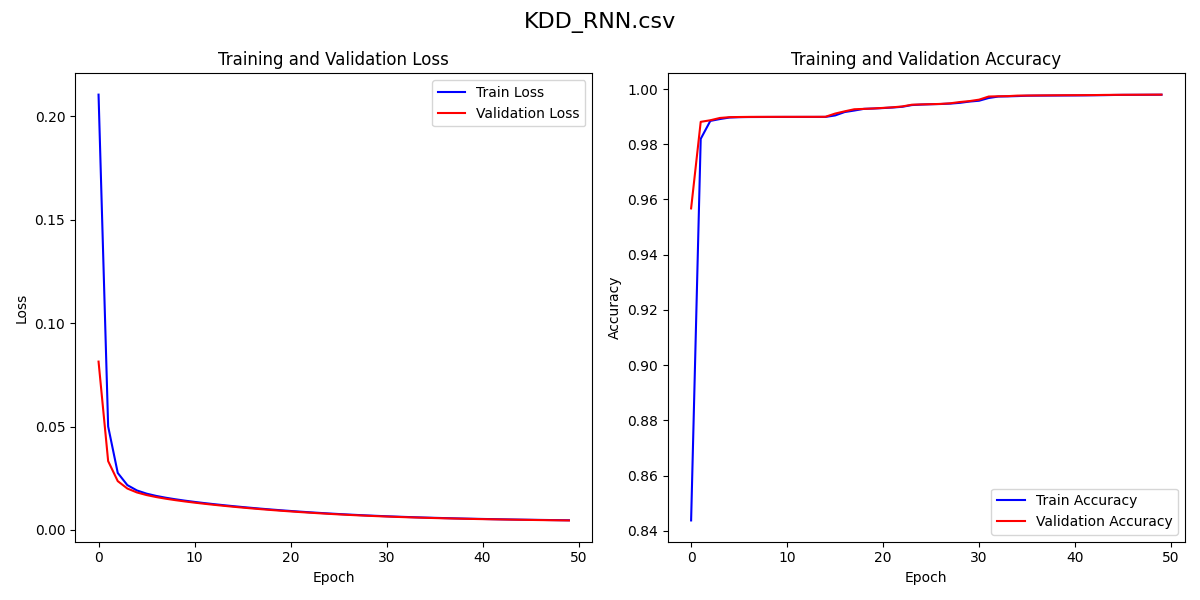
\includegraphics[width=0.8\textwidth]{img/KDD_RNN.csv.png}
    \caption{Evolución de la Precisión y la Pérdida durante el Entrenamiento del Modelo LSTM.}
    \label{fig:lstm_training_process}
\end{figure}

\subsection{Evaluación del Modelo}

El modelo LSTM se evalúa utilizando el conjunto de datos de prueba, logrando una alta precisión en la detección de diferentes tipos de intrusiones. La matriz de confusión, presentada en la Tabla~\ref{tab:lstm_confusion_matrix}, detalla el rendimiento del modelo en términos de instancias correctamente clasificadas y errores de clasificación en cada clase.

\begin{table}[h]
    \centering
    \begin{tabular}{|c|c|c|c|c|c|}
        \hline
        \textbf{Clase Real} & \textbf{DoS} & \textbf{Probe} & \textbf{R2L} & \textbf{U2R} & \textbf{Normal} \\
        \hline
        \textbf{DoS} & 1,165,359 & 1 & 0 & 0 & 13 \\
        \hline
        \textbf{Probe} & 5 & 12,293 & 1 & 0 & 100 \\
        \hline
        \textbf{R2L} & 1 & 0 & 269 & 0 & 79 \\
        \hline
        \textbf{U2R} & 0 & 0 & 0 & 0 & 9 \\
        \hline
        \textbf{Normal} & 42 & 7 & 50 & 0 & 291,391 \\
        \hline
    \end{tabular}
    \caption{Matriz de Confusión para la Clasificación Multiclase en el Conjunto de Prueba del Modelo LSTM.}
    \label{tab:lstm_confusion_matrix}
\end{table}

\subsection{Conclusiones}

La arquitectura RNN-LSTM propuesta ha demostrado ser eficaz en la detección de intrusiones en redes. La capacidad de las LSTM para capturar dependencias temporales complejas en los datos secuenciales permite una clasificación precisa y robusta de diferentes tipos de intrusiones. El enfoque basado en secuencias temporales mejora la detección de patrones de intrusión recurrentes y la capacidad del modelo para generalizar a nuevas situaciones.







En el articulo \citep{elmasry2019empirical} están los experimentos con DNN, RNN,  RBM que puedo tomar también como referencia porque está muy bien explicado las capas e hiperparámetros que utiliza.



Para evaluar el rendimiento del autoencoder convolucional en el problema de Microsoft Malware Clasification, se ha generado una matriz de confusión con los datos de prueba. 


\begin{figure}[H]
    \centering
    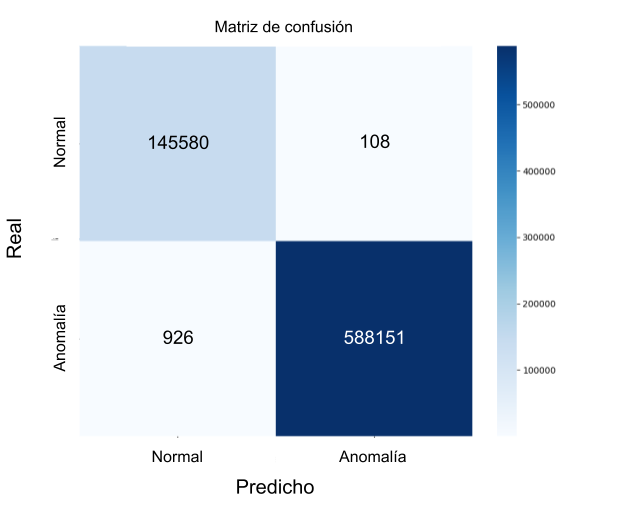
\includegraphics[width=0.6\textwidth]{img/confusionMatrixCNN_KDD.png}
    \caption{Matriz de confusión del modelo utilizando una CNN.}
    \label{fig: cnnKDDConfusion}
\end{figure}


En ella se puede observar como la mayoría de las predicciones están bien clasificadas al igual que para la \acrshort{cnn}, pero la clase con etiqueta 5 obtiene un 33\% de éxito también.
 
Además en la tabla \ref{tab:metrics}, se puede observar una alta precisión y sensibilidad en la mayoría de las clases, con F1-scores que oscilan entre 0.89 y 0.98 para las clases 1, 2, 3, 4, 6, 7, 8 y 9, lo que indica un gran equilibrio entre la precisión y la sensibilidad. La clase 3 sobresale con un F1-score de 0.98, reflejando una excelente precisión (0.97) y sensibilidad (0.99). Sin embargo, la clase 5 presenta un rendimiento significativamente inferior, con una precisión de 0.49, una sensibilidad de 0.33 y un F1-score de 0.39, señalando que el modelo tiene dificultades en identificar correctamente los ejemplos de esta clase. 


\begin{table}[H]
\centering
\begin{tabular}{|c|c|c|c|c|}
\hline
Clase & Precisión & TPR (Sensibilidad) & FPR & F1 Score \\ \hline
1 & 0.94 & 0.97 & 0.06 & 0.96 \\ \hline
\end{tabular}
\caption{Métricas de rendimiento de la CNN.}
\label{tab:kddCNN}
\end{table}

Este problema, al igual que en el caso de la \acrshort{cnn}, se podría resolver usando pesos de clase. 



\end{comment}